
\section{Experimentalism}
\begin{frame}
  \begin{center}
    Part II: Experimentalism
  \end{center}
\end{frame}

\subsection{The role of an experiment in science}

\begin{frame}{The Role of Experiments in Science}
  \begin{columns}
    \column{.5\textwidth}
      Experiments occupy a central role in science.
      They are how we obtain information that help us answer our scientific
      questions.

      \bigskip

      So let's talk about what is an experiment, in detail.
    \column{.5\textwidth}
      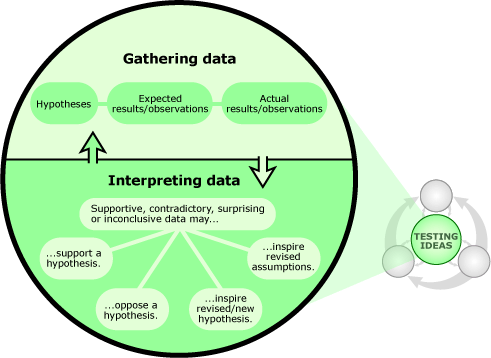
\includegraphics[width=1\textwidth]{../img/understandingscience_zoom2}
  \end{columns}
\end{frame}

\begin{frame}{The Role of Experiments in Science}{Philosophy and Experimentalism}
  \begin{columns}
    \column{0.8\textwidth}
    \begin{itemize}
      \item Philosophy of science: How can we know things?
      \begin{itemize}
        \item Can we know things through logic? Can we trust our senses? Is knowledge immutable? etc.
      \end{itemize}\bigskip

      \item According to Popper, the only way to obtain knowledge about the world is through rigorous experimentation (\structure{Experimentalism});
      \begin{enumerate}
        \item Formulate a question as a \structure{scientific hypothesis};
        \item Execute an experiment following the hypothesis;
        \item Support or reject the hypothesis;
      \end{enumerate}\bigskip

      \item The definition of \structure{scientific hypothesis} is important. In Experimentalism, a scientific hypothesis is one that \structure{produces falsifiable predictions}.
    \end{itemize}

    \column{0.2\textwidth}
    \includegraphics[width=1\textwidth]{../img/wikipedia_popper}\\
    Karl Popper (1902--1994)
    \ppagenote{Karl Popper picture from Wikipedia}
  \end{columns}
\end{frame}

\begin{frame}{Not everyone agrees with Popper, though...}
  \begin{center}
    \includegraphics[width=0.7\textwidth]{../img/existentialcomics_popper}
    \ppagenote{"Freud and Popper" from \url{http://existentialcomics.com/}}
  \end{center}
\end{frame}

\subsection{Characteristics of an experiment}
\begin{frame}{Defining a "fair" experiment}
  Generally, we are interested in a "fair" experiment, that provides new evidence
  for the scientific question that we are trying to answer. A fair experiment has the following characteristics:\vfill

  \begin{itemize}
    \item It provides something to compare against;\medskip
    \item It controls the variables of interest;\medskip
    \item It avoids bias in the results;\medskip
    \item It is reproducible;\medskip
    \item It separates chance results from real differences;
  \end{itemize}
\end{frame}

\subsection{1. Provides something to compare against}
\begin{frame}{"Provides Something to Compare Against"}{Scientific Hypothesis}

  A \structure{scientific hypothesis} is the question that we try to answer with an experiment. For an experiment to be useful, it is necessary that it has at least two possible results. Afterall, if you already know the result of your experiment, why do it?
  \vfill

  Examples of scientific hypothesis:
  \begin{itemize}
    \item {\bf Comparing different systems:}\\
    Chocolate cookies taste better than mint.
    \item {\bf Comparing explanations to a phenomenom:}\\
    Bananas turn black in the refrigerator because of bacteria, not the temperature.
    \item {\bf Test the characteristic of a system:}\\
    One apple tree is enough to feed our home for the entire year.
  \end{itemize}\bigskip
\end{frame}

\begin{frame}{Scientific Hypothesis}{Specific Hypothesis}
  One characteristic of good scientific hypothesis is that they are \structure{specific}. The more detail you give to the question you want to answer, the easier it is to design a good experiment:\bigskip

  Example:
  \begin{itemize}
    \item "my Optimization method is the best!"
    \item "The optimization method proposed in this paper is better than existing methods!"
    \item "Using Polynomial mutation is better than gaussian mutation for optimization methods!"
    \item "Polynomial mutation increases the convergence rate of an optimization method, when compared to gaussian mutation!"
  \end{itemize}
\end{frame}

\begin{frame}{Scientific Hypothesis}{Falsifiable Hypothesis}
  Another important characteristic of good scientific hypothesis is that they are \structure{falsifiable}. A falsifiable hypothesis is one that {\bf could be proven false}, depending on the result of the experiment.\bigskip


  \begin{itemize}
    \item \alert{Non Falsifiable Hypothesis:} "This Neural Network can solve any problem if we find the right parameters".\\
    {\smaller
    If the method does not solve the problem, it just means that the parameters are wrong, so we do another experiment... and another... and another...}\bigskip

    \item \structure{Falsifiable Hypothesis:} "Using algorithm A and parameters $\theta$, we achieve a speed-up of 1.5 on benchmark B."
  \end{itemize}\bigskip
\end{frame}

\subsection{2. Controlling Variables Of Interest}
\begin{frame}{An experiment control variables of interest}{Types of Experiments}
  There are many \structure{variables} that affect the result of an experiment. For example, if you want to test if chocolate ice cream tastes better than coffee, the result may be different if you ask children or PhD students.\bigskip

  If your scientific question is focused on the opinions of PhD students (WHY?), you can control the variables of the experiment, and not include children or professors in your survey.\bigskip

  Depending on how much freedom you have to control the variable in your experiments, we can classify experiments in three types:
  \begin{itemize}
    \item Observational Experiments;
    \item Retrospective Experiments;
    \item Controlled Experiments;
  \end{itemize}
\end{frame}
%% Three types of data collection

\begin{frame}{Types of Experiments}{Observational Experiments}
  In an \structure{Observational Experiment}, you obtain data by observing a phenomena without interacting with it directly.
  \bigskip

  {\bf Example:} you count the number of people who use the train with and without masks every day.
  \bigskip

  \begin{itemize}
    \item Requires care to observe representative situations;
    \item Allows the researcher to choose general conditions for observation;
    \item The situation of interest may be too rare to observe naturally;
  \end{itemize}
\end{frame}

\begin{frame}{Types of Experiments}{Retrospective Experiments}
  In a \structure{Retrospective Experiment}, the researcher obtains data from historical records (newspaper, reports, other scientific papers).\bigskip

  {\bf Example:} you search from the relationship between announcements of celebrity marriages, and total number of registered marriages;\bigskip

  \begin{itemize}
    \item Generally cheaper, and may be the only way to gather data over a very long period of time;
    \item Susceptible to missing records or bias in recording;
  \end{itemize}
\end{frame}

\begin{frame}{Types of Experiments}{Controlled Experiments}
  In a \structure{Controlled Experiment}, the researcher is able to define several variables in the experiment, and perform it in the conditions desired.\bigskip

  {\bf Example:} You develop a new algorithm, and test it on some selected data sets, on a collection of different computational architectures;\bigskip

  \begin{itemize}
    \item Gives a lot of control for the researcher;
    \item If not designed carefully, allows for the introduction of biases into the experiment;
    \item Can be the most expensive kind of experiment (although not always in CS);
  \end{itemize}
\end{frame}


\subsection{3. Controlling For Bias}

\begin{frame}{3. A fair experiment control for biases}
  \begin{block}{}
    \hfill "With great power comes great responsibility"
  \end{block}\bigskip

  When you \structure{control the variables} of your experiment ({\bf or when you don't!}). You can introduce biases to the result.\bigskip

  For example, if you compare the speed of two computer programs, it may be hard to see a difference, if you run your experiment in a very powerful computer. Or the difference may be exaggerated if you use a very slow one.\bigskip

  To have a fair experiment, it is important to be aware of these source of biases, and change your experiment to avoid those biases. This is one of the main tasks of \structure{Experimental Design}.
\end{frame}

\begin{frame}{Some Experiment Design Questions}
  \begin{itemize}
    \item Which methods we compare in the experiment?
    \item Which data sets are used?
    \item How many times do we interview each participant?
    \item In what order do we perform the experiments?
    \item Which data is reported, and how is the data summarized?
    \item What criteria determines that the hypothesis was accepted or rejected?
    \item What hyper-parameters do we use?
    \item How many times is the experiment repeated? How are these repetitions sumarized?
  \end{itemize}
\end{frame}

%% TODO: Talk about techniques for experiment design (Educated Guesses, Factorial Design, OVAT, etc -- maybe in lecture 2 or later)

\begin{frame}{Experiment Design}{Example: Controlling for Variation}
  \hfill\includegraphics[width=.2\textwidth]{../img/pixabay_clock}

  Let's say you are comparing two computer programs by measuring their running time (wallclock time).
  \bigskip

  You know that the running time of a program is affected by other programs that are running in the background of the operational system. For example, if a software update happens in the background, it could make a run much slower.
  \bigskip

  To control for this variation, you make sure to run your experiment in a system with a minimum number of running processes, and you also repeat the experiment many times and take the average running time;
  \ppagenote{Clock image from \url{https://pixabay.com}}
\end{frame}

\begin{frame}{Experiment Design}{Example: Controlling for Independence}
  Imagine that you are comparing two website designs with the following experiment: You measure the time for a user to find some information on website A, then you measure the time for website B. \bigskip

  If you make this comparison always in the same order for all users, you discover that the users are a bit faster for website B, because they get used to the testing environment and are more relaxed. \bigskip

  To remove this influence, you make sure that the test order is always random, or you make sure that each user tests only one website.

  \begin{center}
    \includegraphics[width=0.2\textwidth]{../img/irasutoya_website1}\hspace{1cm}
    \includegraphics[width=0.2\textwidth]{../img/irasutoya_website2}
    \ppagenote{Website images from \url{https://www.irasutoya.com}}
  \end{center}
\end{frame}

\begin{frame}{Experiment Design}{Example: Controlling for Fairness}
  You propose a neural network architecture for a new vision problem, and you compare it against traditional architectures.\bigskip

  Because of the special characteristics of the problem, you fine-tune the hyper-parameters of your architecture to achieve the best performance.\bigskip

  To make sure that the comparison is fair, you use the same fine-tune techniques to the traditional architecture that you are comparing against, not using its old hyper-parameters from the literature.

  \hfill\includegraphics[width=0.2\textwidth]{../img/pixabay_neuralnetwork_gordonjohnson}
  \ppagenote{Neural Network image by Gordon Johnson from \url{https://pixabay.com}}
\end{frame}

\begin{frame}{Pre-registered Experiments}
  Pre-registration is the act of fully defining your research protocol {\bf before you begin to collect or analyze data}.
  \bigskip

  By pre-registering your research, you avoid modifying your methods to fit your hypothesis (or modifying your hypothesis to fit your data)
  \bigskip

  Public pre-registration can prevent the loss of negative results. Private pre-registration can help you keep yourself in check.\bigskip

  \begin{columns}
    \column{.7\textwidth}
    Learn more: Center for Open Science \url{https://cos.io/prereg/}
    \column{0.3\textwidth}
    \includegraphics[width=1\textwidth]{../img/prereg-badge}
  \end{columns}
\end{frame}

\subsection{4. It is reproducible}
\begin{frame}{Reproducible Experiments}
  Reproducibility is an important property of a good experiment:
  \bigskip

  \begin{itemize}
    \item Others can confirm your results;
      \medskip
    \item Others can build on your results;
      \medskip
    \item Others can improve your results;
      \medskip
    \item Society can use your results;
  \end{itemize}
\end{frame}

\begin{frame}{Reproducible Experiments}{How can we make experiments more reproducible?}
  \begin{exampleblock}{Clear Experiment Design}
    Detailed steps taken to perform the experiment; Values of relevant parameters; How the results are processed and evaluated;
  \end{exampleblock}
  \begin{exampleblock}{Open Data and Open Source}
    Data acquisition protocol is clearly defined; Raw data and pre-processing scripts are available; Data is well documented;\bigskip

    For CS, open source of proposed algorithms is essential;
  \end{exampleblock}
  \begin{exampleblock}{Open Documentation}
    Code used for statistical analysis and data visualization;
  \end{exampleblock}
\end{frame}

\subsection{5. Separates chance from reality}
\begin{frame}{A good experiment separates chance from reality}
  Experiments in the real world almost never give exactly the same result, even when perfectly replicated.\bigskip

  These \structure{sources of noise} can hide the real truth of a scientific question behind a coincidence, or a spell of bad luck.\bigskip

  Over the years, the field of statistics has developed many techniques to measure how much an experiment can be influenced by luck, and how to separate coincidences from real differences.\bigskip

  This will be the topic of our future classes.
\end{frame}

\subsection{In short}
\begin{frame}{Summary}
  Many scientific discoveries and scientific advancements (as well as your own master thesis!) depend on good experiments and data collection.\bigskip

  Unfortunately, good experiments are not as simple as simply going out on the streets and start collecting data.\bigskip

  Careful planning is necessary, not only to make sure that your experiment is not affected by biases, but also to make sure that your experiment is able to answer the question that you are asking.\bigskip

  {\bf Experiment Design} is the proccess of carefully planning an experiment to make sure that it is fair and effective.
\end{frame}
